%Related work
\section{Literature review}\label{sec:lit}%

In the early 20th century \cite{fisher1911equation,fisher1922purch} spawned an extensive literature in
monetary economics based on what he called the equation of exchange, in which
velocity played a crucial role.  Since this literature does not relate to
account for the information blockchains make available, and is reviewed at
length by \cite{friedman2017quantity} we restrict our review to the
literature on the velocity of cryptocurrencies.  Both theoretical pricing
models and empirical studies of price determinants have addressed velocity.

Empirically, \ac{cdd} is commonly used as proxy variable in regressions of
cryptocurrency return patterns. %
Based on the quantity equation, these studies expect a significant positive
relationship between prices and their chosen proxy. %
While \cite{kancs2015digital} and \cite{ciaian2016digital} confirm the
hypothesis, more often it is rejected
\citep{deleo2014does,georgoula2015using,bouoiyour2015does,ciaian2016economics,luis2019drivers}.
Following \cite{fisher1911equation}, \cite{athey2016bitcoin} estimate
velocity as the ratio of adjusted on-chain transaction volume to the total
Bitcoin supply when modeling the bitcoin price. %%% assuming constant velocity. --> I don't
                                %%% understand: that would NOT be constant? %
Additionally they employ the ratio of off-chain transaction volume and coin
supply (both denominated in USD) as a velocity estimator. %
% \cite{deleo2014does}, to the best of our knowledge, were the first to explore the relationship between cryptocurrency prices and the velocity of money. %
% The analysis adopted \ac{cdd}%
% as velocity approximation, used a simple multiple regression analysis and did find a significant negative relationship to Bitcoin returns. %
% \cite{georgoula2015using} conducted a time series analysis using support vector machine learning (SVM) and sentiment indicators but also technological and economic variables. %
% Using the same proxy-variable as \cite{deleo2014does}, the authors did not find %
% a significant relation between velocity and Bitcoin returns. %
% \cite{bouoiyour2015does} analyzed Bitcoin prices using an \ac{ardl} model and a variety of technical and behavioral variables. %
% Velocity was again approximated by \ac{cdd} and found to have %
% no significant relation to Bitcoin returns. %
% \cite{ciaian2016economics} analyzed Bitcoin price formation using an adaption %
% of Fisher's quantity theory to the gold standard, \cite{barro1979money}, for variable selection and applied vector autoregressive (VEC) and \ac{ardl} models. %
% The authors again used \ac{cdd} as velocity approximation %
% and did not find a significant relationship either. %
% \cite{luis2019drivers}, using the same proxy-variable, differentiate between long- and short-run price %
% formation for Bitcoin and attempt to disentangle the use of Bitcoin as %
% medium-of-exchange and speculative asset. %
% The authors tested the effect of velocity for long term price determination but did not find statistic significance. %


Theoretically, \cite{bolt2016value} use velocity as central building block of
their pricing model. %
They decompose the velocity of money into a part for monetary units used as
media of exchange and a part for those used as long-term investment. %
The paper does not specify, however, how this decomposition could be
implemented. %
Our paper is the first to offer an operationalization for UTXO-based
cryptocurrencies.%

In \cite{athey2016bitcoin} a measure of velocity of Bitcoin
acknowledging the need for adjustments addressing the transaction volume
generated by change transactions is presented. %
\cite{kalodner2017blocksci} adopt the same concept but provide deeper
insights into its technical configuration as a byproduct of introducing a new
blockchain parser for UTXO-based cryptocurrencies. %
% We root their approach in monetary theory and compare their measure to common proxy-variables and the new %
% measure of velocity based on a segregated money supply. %
%

\begin{figure*}
  \centerline{%
    \ifdefined\varInputFigs%
    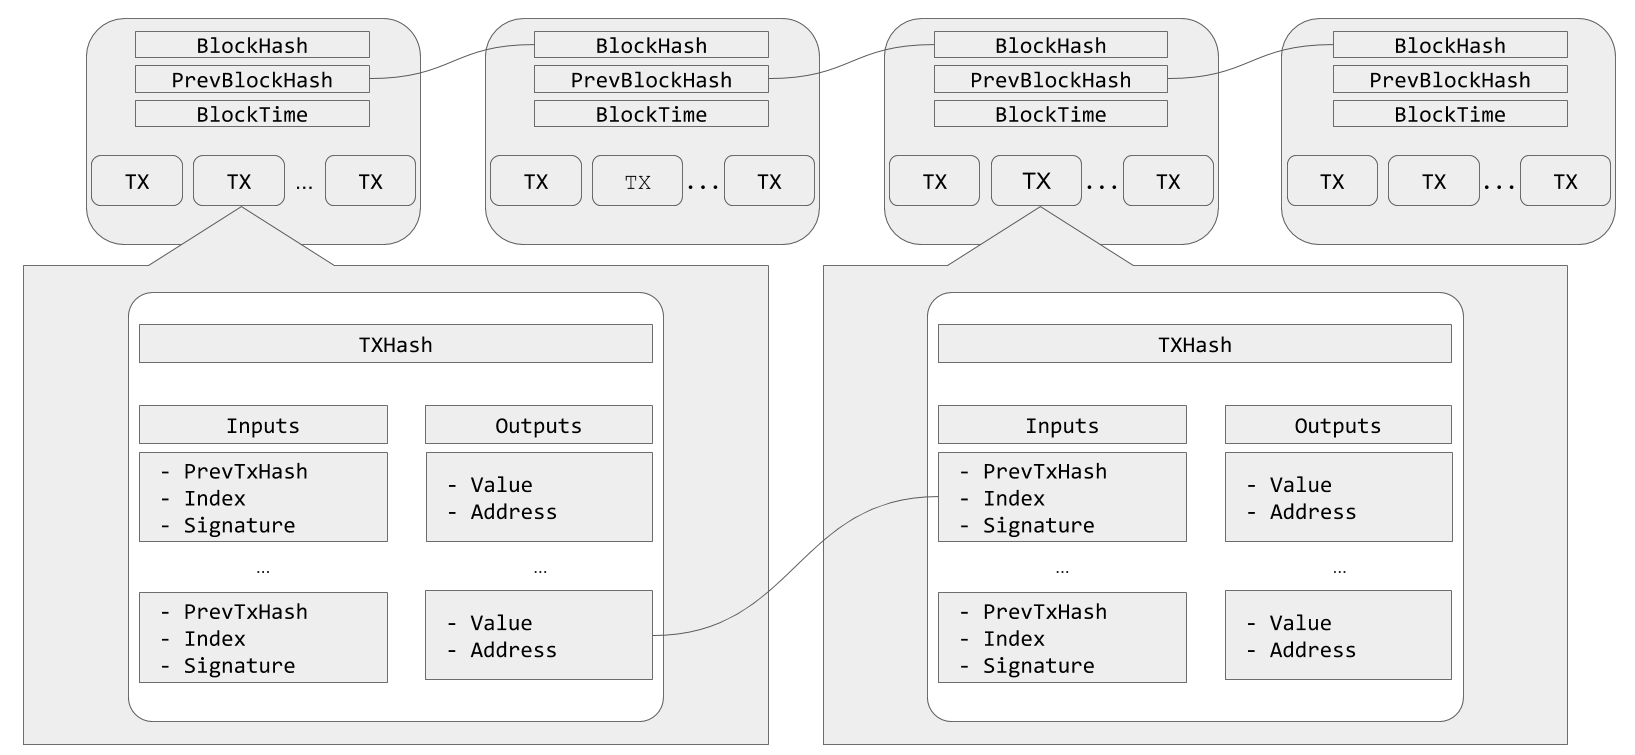
\includegraphics[width=0.8\linewidth]{fig/utxo_sys_HR}%
    \else%
    \fi%
  }%
  \caption{Blockchain and Transactions (adapted from \cite{tschorsch2016bitcoin}).}
  \label{fig:utxo_sys}
\end{figure*}

Recognizing the need for a more precise method, \cite{smith2017bitcoin} proposed
a cryptocurrency's \textit{turnover} as derivation of \ac{cdd}. %
We compare this approach to the other methods and show that, compared to
\ac{cdd}, the measure is indeed closer to the velocity estimates in many
tests. %




%%% Local Variables:
%%% mode: latex
%%% TeX-master: "../main"
%%% End:
